\documentclass[sigconf]{acmart}

\AtBeginDocument{%
	\providecommand\BibTeX{{%
		Bib\TeX}}}

\usepackage{graphicx}
\usepackage{amsmath}
\usepackage{placeins}

\begin{document}

\title{Project Progress Report: Improving RUNG for Robust Graph Aggregation}

\author{Tawkir Aziz Rahman \\ 2005090}
\affiliation{%
	\institution{Bangladesh University of Engineering and Technology}
	\city{Dhaka}
	\country{Bangladesh}
}

\author{Dipanta Kumar Roy Nobo \\ 2005074}
\affiliation{%
	\institution{Bangladesh University of Engineering and Technology}
	\city{Dhaka}
	\country{Bangladesh}
}

\renewcommand{\shortauthors}{Project Team}

\begin{abstract}
This report presents our project progress on improving RUNG (Robust UNbiased Neighborhood Graph aggregation) for robust Graph Neural Networks under Adaptive Attack settings. We start from the RUNG 2024 NeurIPS foundation and test three improvements: Percentile Gamma, Parametric Gamma, and Learnable Cosine Distance, followed by a combined model. We compare behavior on homophilic and heterophilic datasets, discuss what is working now, and list the remaining gaps we plan to address before the final project presentation.
\end{abstract}

\ccsdesc[500]{Computing methodologies~Learning from graph data}
\ccsdesc[300]{Security and privacy~Adversarial learning}

\keywords{Graph Neural Networks, RUNG, RUGE, Adaptive Attack, Estimation Bias, Percentile Gamma, Parametric Gamma, Learnable Distance, Heterophily}

\maketitle

\section{Introduction}
The base paper for this project is RUNG 2024 NeurIPS, ``Robust Graph Neural Networks via Unbiased Aggregation'' \cite{hou2024rung}. RUNG means Robust UNbiased Neighborhood Graph aggregation. It is designed for robust graph aggregation techniques for Graph Neural Networks.

The core problem is that many GNNs can face adaptive attacks. Attackers can add fake edges among nodes and disrupt the result. Many graph signal estimators exist and do work, but they fail badly in one case: when the attacker knows the model and the dataset. If the attacker knows the parameters, they can attack in an adaptive way and break those defenses.

Previous defenses include two regularization styles, often described as \(\ell_1\) and \(\ell_2\) defense. The \(\ell_1\) defense uses an absolute penalty, while \(\ell_2\) uses a squared penalty. In both styles, the algorithm checks edges and assigns weights. Suspicious edges get larger penalties so they cannot hurt the graph as much.

The problem appears when the attack budget is high, meaning the attacker can inject many fake edges. Even after weighting and penalizing, those fake edges still influence the final aggregation and shift the estimate. This is the Estimation Bias problem \cite{fan2001}. For \(\ell_1\) penalty, the values still pull the estimate over time. For \(\ell_2\), the shift is often worse because squared penalties can deviate further from the original signal.

RUNG addresses this with an unbiased strategy. Instead of only reducing suspicious edge weights, it can force them to zero if they are highly suspicious. The goal is Unbiased Aggregation: if an edge crosses a suspicious threshold, sever it completely.

RUNG does this through the Robust and Unbiased Graph signal Estimator (RUGE) \cite{hou2024rung}. The estimator uses MCP-based weighting to decide whether an edge should contribute or be pruned:

\begin{equation}
\arg\min_{\mathbf{F}}\,\mathcal{H}(\mathbf{F})=
\sum_{(i,j)\in\mathcal{E}}\rho_{\gamma}\left(\left\lVert\frac{\mathbf{f}_i}{\sqrt{d_i}}-\frac{\mathbf{f}_j}{\sqrt{d_j}}\right\rVert_2\right)
+\lambda\sum_{i\in\mathcal{V}}\lVert\mathbf{f}_i-\mathbf{f}^{(0)}_i\rVert_2^2
\label{eq:ruge_obj}
\end{equation}

\begin{equation}
\rho_{\gamma}(y)=
\begin{cases}
y-\dfrac{y^2}{2\gamma}, & y<\gamma\\
\dfrac{\gamma}{2}, & y\ge\gamma
\end{cases}
\label{eq:mcp_penalty}
\end{equation}

The MCP form in Eq.~\ref{eq:mcp_penalty} follows the same non-convex penalty family discussed in statistical learning \cite{fan2001} and is the key reason RUGE can reduce bias while preserving robust behavior. This is the foundation we built on in our project.

\section{Materials and Methods}
\subsection{Datasets}
We evaluate on homophilic datasets (Cora, Citeseer, Pubmed) and heterophilic datasets (Cornell, Wisconsin, Chameleon). The heterophilic benchmarks are standard in Geom-GCN \cite{pei2020geomgcn}. We included them because the base RUNG paper is mainly stronger for homophilic graphs, and we wanted to test what happens when class-connected neighbors are less similar.

\subsection{Base Architecture and Training Context}
Our starting point is the RUNG architecture with the RUGE estimator and MCP penalty \cite{hou2024rung}. The training setup follows the same robust aggregation idea under Adaptive Attack conditions. In our progress stage, we focused on modifying the thresholding and distance components while keeping the core backbone stable.

\subsection{Method 1: Percentile Gamma}
Our first target was changing gamma in the RUGE estimator. In original RUNG, gamma is selected early and kept fixed across layers. The issue is that with deeper GNN layers, node features become smoother and pairwise differences become smaller, a standard oversmoothing behavior \cite{li2018deeper}. If gamma stays fixed, deeper layers can treat too many edges as valid.

To fix this, we implemented Percentile Gamma. Gamma is adapted per layer using a percentile-based threshold over edge differences. As differences shrink, gamma also shrinks. Attack edges usually connect dissimilar nodes, so they appear in the high-difference tail. We prune edges above a selected \(q\)-percentile rule. We can choose aggressive pruning (e.g., 50\%), moderate (75\%), or conservative (95\%). In this report, we use \(q=0.75\) as the normal setting.

\subsection{Method 2: Parametric Gamma}
Second, we implemented Parametric Gamma. Percentile Gamma estimates threshold from current layer statistics. Parametric Gamma instead enforces a predictable decay curve with depth. We set a starting threshold \(\gamma_0\) and a decay multiplier \(r\), then apply:
\[
\gamma_k = \gamma_0\,r^k.
\]

Example with \(\gamma_0=5.0\) and \(r=0.8\): layer 0 is 5.0, layer 1 is 4.0, layer 2 is 3.2, layer 3 is 2.56. This smooth decay follows the same trend as feature smoothing, so the defense remains active at deeper layers where fixed thresholds fail \cite{li2018deeper}.

\subsection{Method 3: Learnable Cosine Distance}
Third, we implemented a learnable defense in RUNG by changing the edge suspiciousness metric. Core RUNG relies on Euclidean distance, which depends strongly on magnitude. Under Adaptive Attack, a malicious node can be crafted to mimic magnitude and reduce Euclidean gap, so poisoned edges can pass through.

We moved to cosine-based distance and made it learnable through a trainable projection matrix before cosine computation. In simple terms, the model learns a custom feature space and then compares directional similarity there. This helps separate useful structural signals from noisy features. The idea is aligned with graph structure learning directions in robust GNN literature \cite{jin2020prognn}.

\subsection{Combined Model Design}
After testing each method separately, we combined them to test unified improvement. The combination is not a direct conflict between Percentile Gamma and Parametric Gamma. We do not apply parametric decay directly to raw distance threshold. Instead, we apply parametric decay to the percentile level \(q\).

In pure Percentile Gamma, \(q\) is fixed for all layers. In the combined design, \(q\) decays with depth, so pruning gets stricter in deeper layers. Parametric Gamma controls aggressiveness over depth, while Percentile Gamma controls how many high-difference edges are pruned per layer.

Learnable Cosine Distance complements this by measuring angle-based feature inconsistency rather than magnitude-only mismatch. That made the model more robust under higher-budget attacks in several settings.

Two design choices explain why we used this exact combination:
\begin{itemize}
\item We did not use only Parametric Gamma + Learnable Distance because learnable distance changes scale during training, while a rigid parametric threshold can become mismatched.
\item We did not use only Percentile Gamma + Learnable Distance with flat \(q\), because this ignores depth-wise oversmoothing and can under-prune or over-prune depending on layer depth.
\end{itemize}

\section{Results and Discussion}
\subsection{Percentile Gamma Results}
For Cora and Citeseer with \(q=0.75\), Percentile Gamma shows improved robustness over base RUNG when attack budget increases.

\begin{figure}[!htbp]
	\centering
	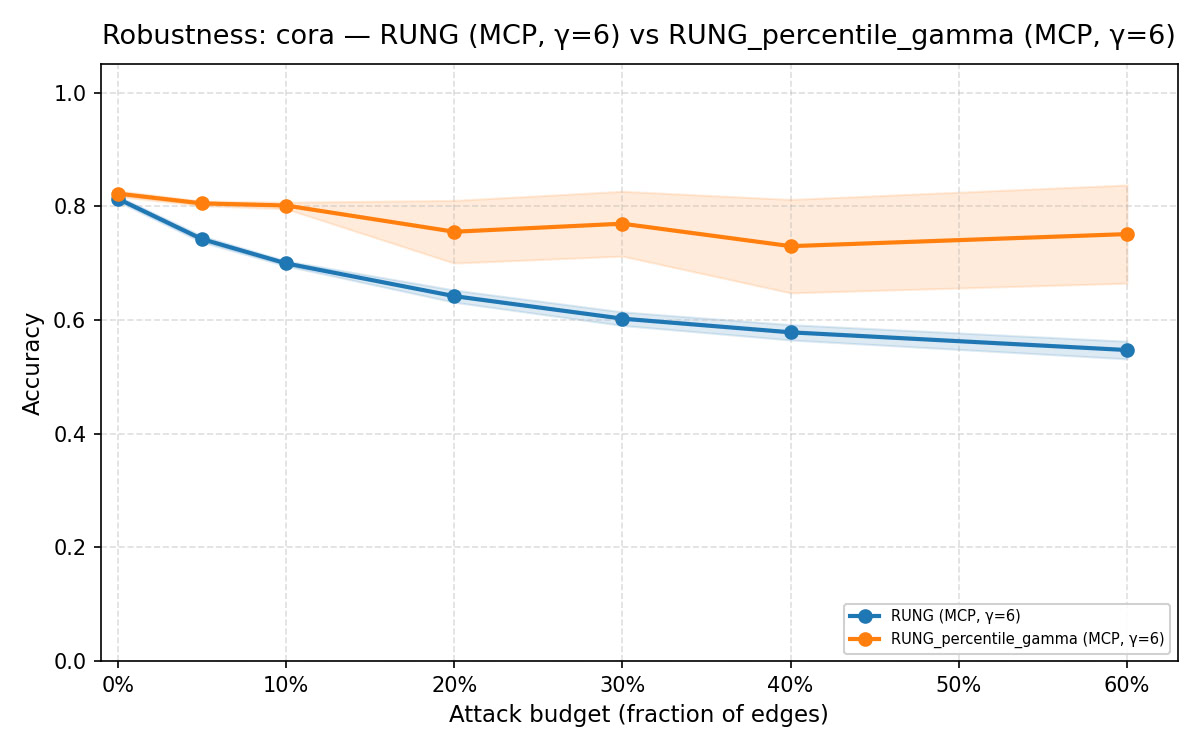
\includegraphics[width=\linewidth]{figures/Cora_RUNG_vs_RUNG_percentile_gamma..jpg}
	\caption{Cora: RUNG vs Percentile Gamma.}
	\Description{Comparison plot on Cora between baseline RUNG and Percentile Gamma method.}
	\label{fig:cora_percentile}
\end{figure}

\begin{figure}[!htbp]
	\centering
	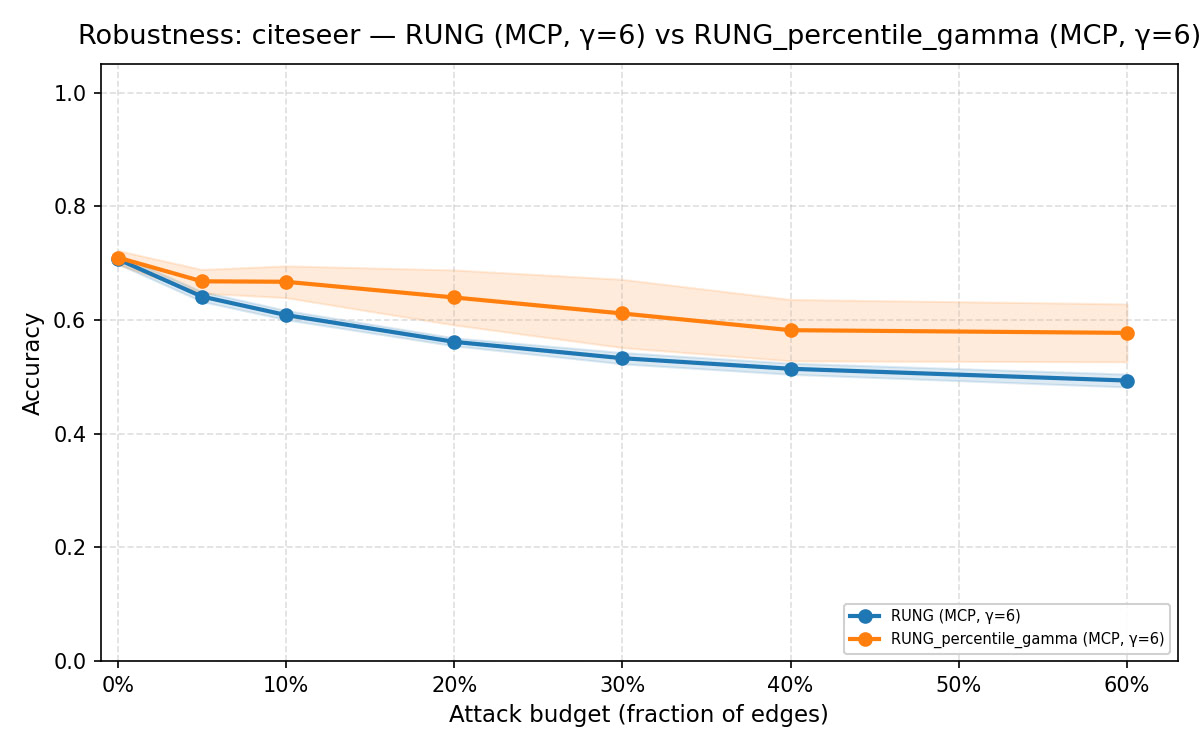
\includegraphics[width=\linewidth]{figures/Citeseer_RUNG_vs_RUNG_percentile_gamma.jpg}
	\caption{Citeseer: RUNG vs Percentile Gamma.}
	\Description{Comparison plot on Citeseer between baseline RUNG and Percentile Gamma method.}
	\label{fig:citeseer_percentile}
\end{figure}
\FloatBarrier

\subsection{Parametric Gamma Results}
On Cora and Citeseer, Parametric Gamma also improves performance over RUNG as attack budget grows. We still observe high variance in some settings, so this method needs more tuning.

\begin{figure}[!htbp]
	\centering
	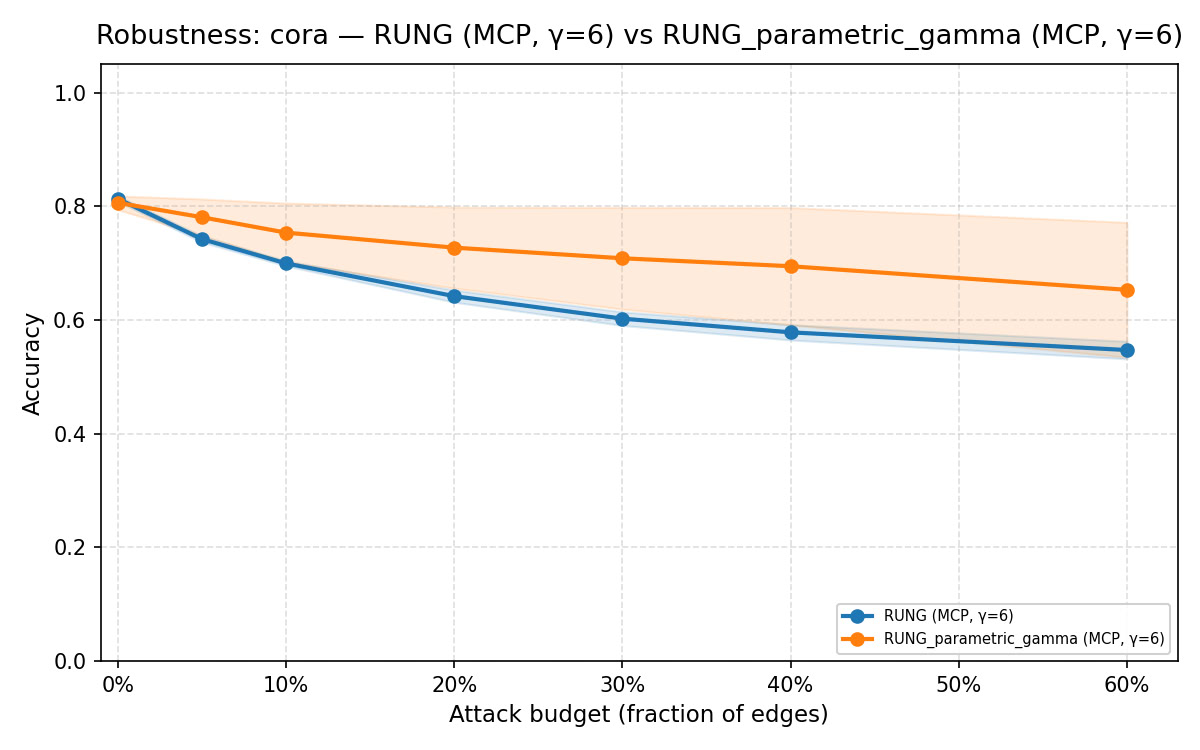
\includegraphics[width=\linewidth]{figures/Cora_RUNG_vs_RUNG_parametric_gamma.jpg}
	\caption{Cora: RUNG vs Parametric Gamma.}
	\Description{Comparison plot on Cora between baseline RUNG and Parametric Gamma method.}
	\label{fig:cora_parametric}
\end{figure}

\begin{figure}[!htbp]
	\centering
	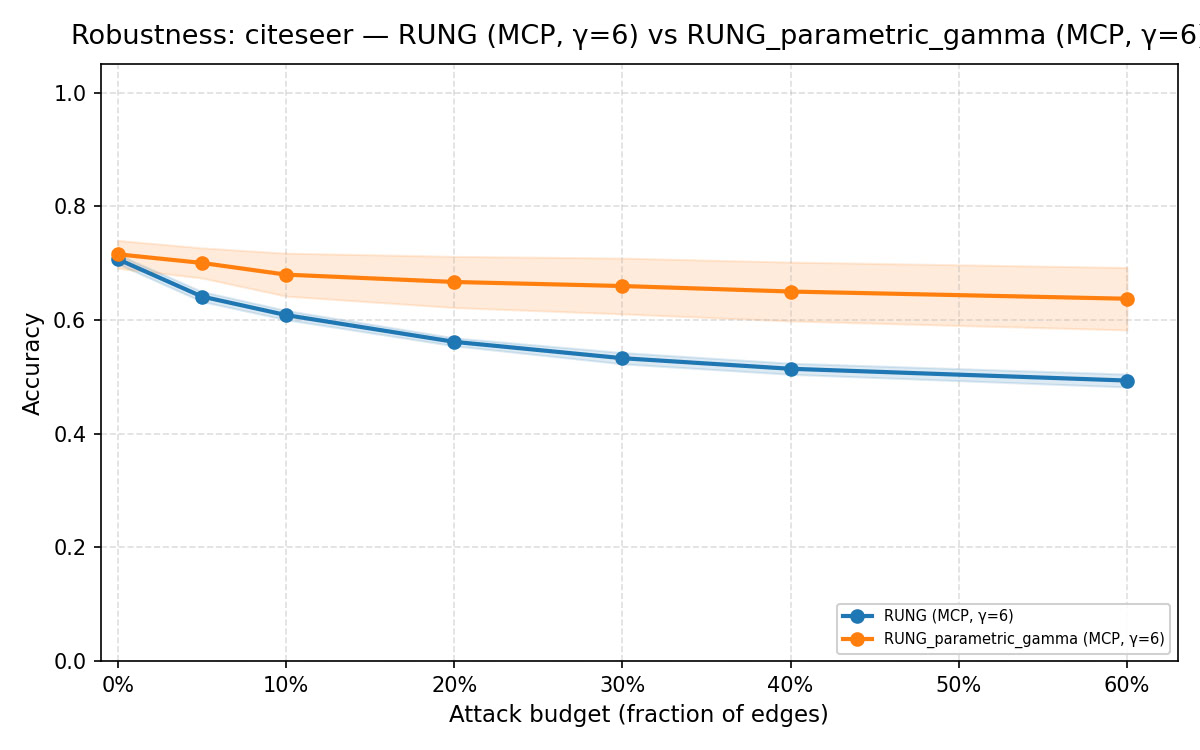
\includegraphics[width=\linewidth]{figures/Citeseer_RUNG_vs_RUNG_parametric_gamma.jpg}
	\caption{Citeseer: RUNG vs Parametric Gamma.}
	\Description{Comparison plot on Citeseer between baseline RUNG and Parametric Gamma method.}
	\label{fig:citeseer_parametric}
\end{figure}
\FloatBarrier

\subsection{Learnable Cosine Distance Results}
Learnable Cosine Distance gives good improvements in several runs. It performs especially well on heterophilic settings where angle-based similarity can preserve useful cross-class structure better than magnitude-based Euclidean distance.

\begin{figure}[!htbp]
	\centering
	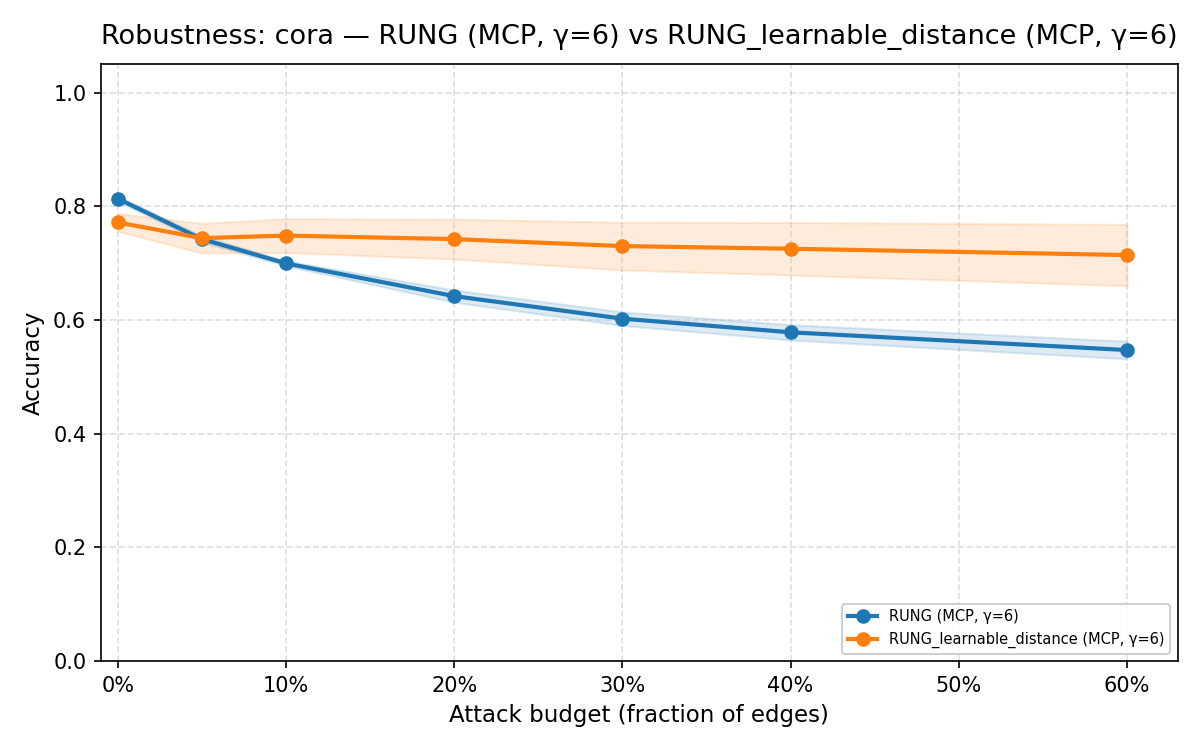
\includegraphics[width=\linewidth]{figures/Cora_RUNG_vs_RUNG_learnable_distance.jpg}
	\caption{Cora: RUNG vs Learnable Cosine Distance.}
	\Description{Comparison plot on Cora between baseline RUNG and Learnable Cosine Distance method.}
	\label{fig:cora_learnable}
\end{figure}

\begin{figure}[!htbp]
	\centering
	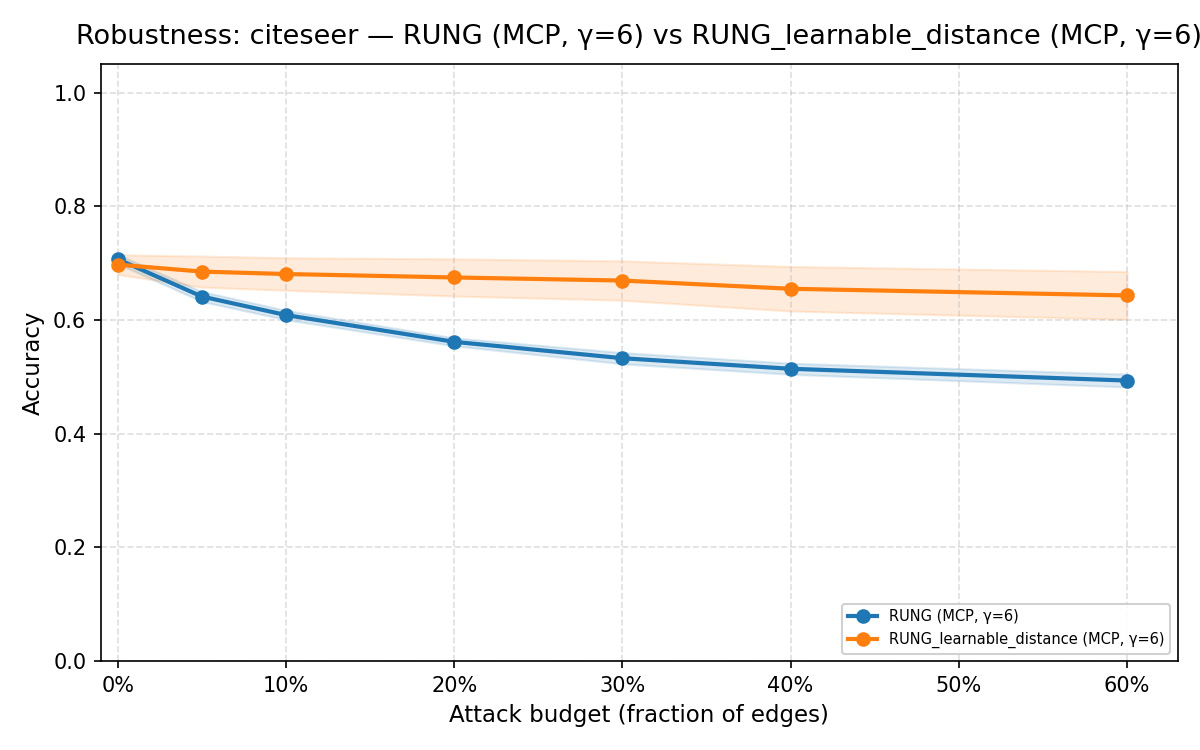
\includegraphics[width=\linewidth]{figures/Citeseer_RUNG_vs_RUNG_learnable_distance.jpg}
	\caption{Citeseer: RUNG vs Learnable Cosine Distance.}
	\Description{Comparison plot on Citeseer between baseline RUNG and Learnable Cosine Distance method.}
	\label{fig:citeseer_learnable}
\end{figure}
\FloatBarrier

\subsection{Combined Model Results}
The combined model was built to test whether the methods strengthen each other under stronger attacks. For homophilic datasets, the combined setup performs very well at higher attack budgets.

\begin{figure}[!htbp]
	\centering
	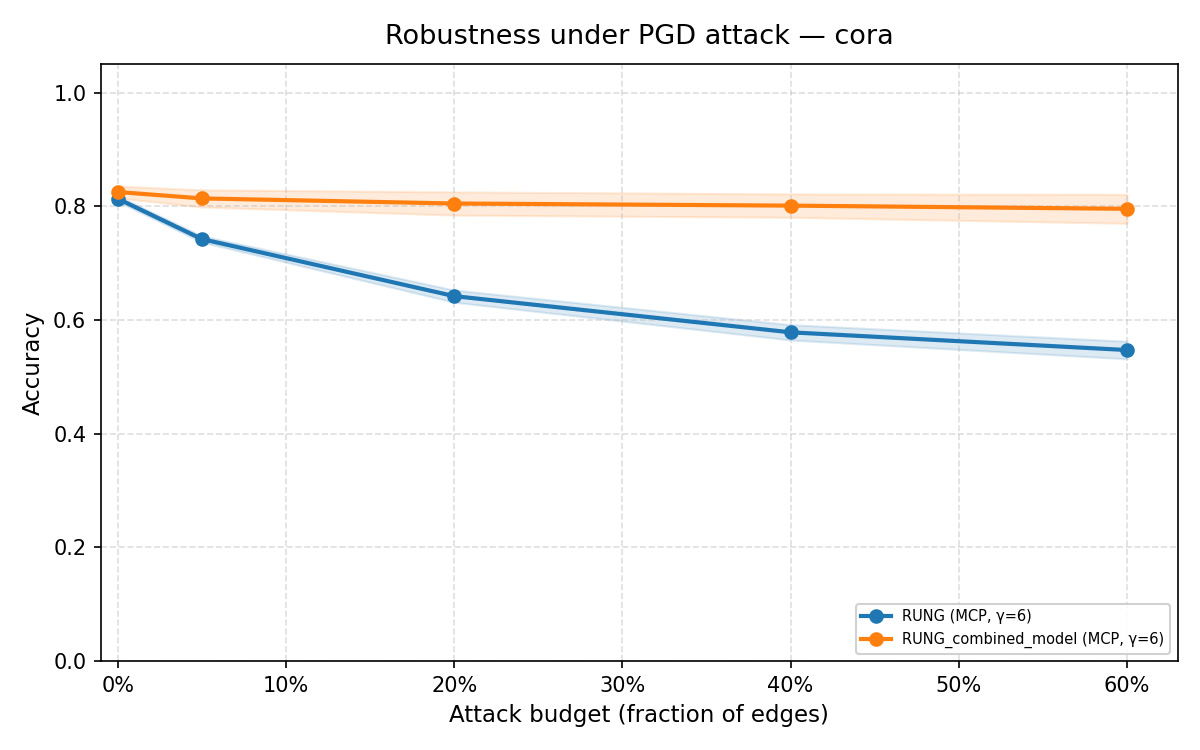
\includegraphics[width=\linewidth]{figures/Cora_RUNG_vs_RUNG_combined.jpg}
	\caption{Cora: RUNG vs Combined Model.}
	\Description{Comparison plot on Cora between baseline RUNG and combined method.}
	\label{fig:cora_combined}
\end{figure}

\begin{figure}[!htbp]
	\centering
	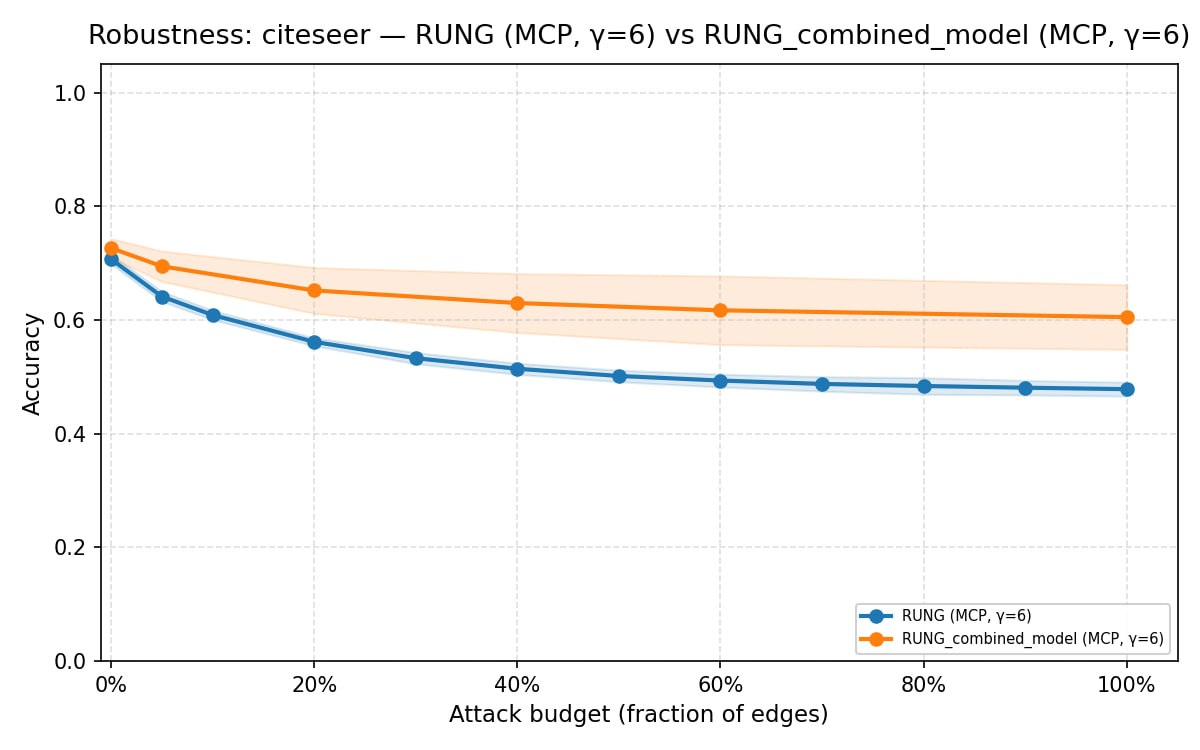
\includegraphics[width=\linewidth]{figures/Citeseer_RUNG_vs_RUNG_combined.jpg}
	\caption{Citeseer: RUNG vs Combined Model.}
	\Description{Comparison plot on Citeseer between baseline RUNG and combined method.}
	\label{fig:citeseer_combined}
\end{figure}

\begin{figure}[!htbp]
	\centering
	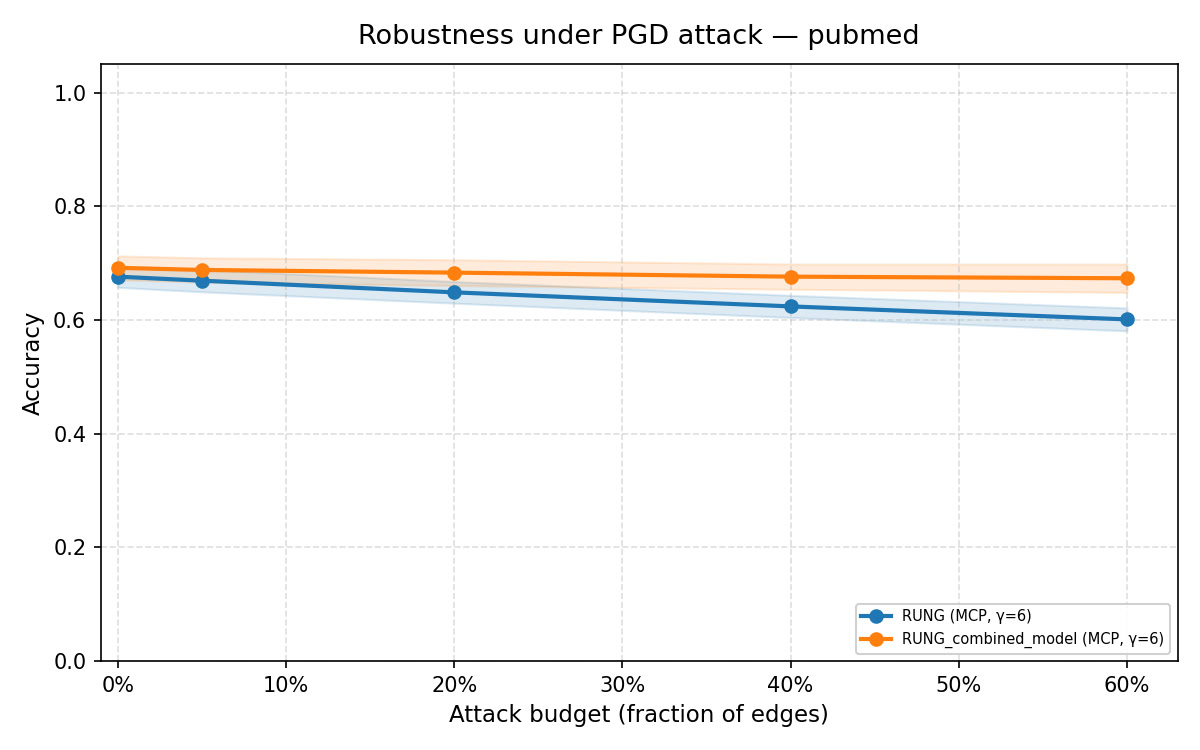
\includegraphics[width=\linewidth]{figures/Pubmed_RUNG_vs_RUNG_combined.jpg}
	\caption{Pubmed: RUNG vs Combined Model.}
	\Description{Comparison plot on Pubmed between baseline RUNG and combined method.}
	\label{fig:pubmed_combined}
\end{figure}
\FloatBarrier

For heterophilic datasets, we observed a different behavior. Learnable Distance can outperform combined thresholding variants in some cases. The combined model is often still better than original RUNG, but not always better than the best independent method. A key reason is over-pruning in heterophilic graphs: valid edges can naturally connect dissimilar nodes.

\begin{figure}[!htbp]
	\centering
	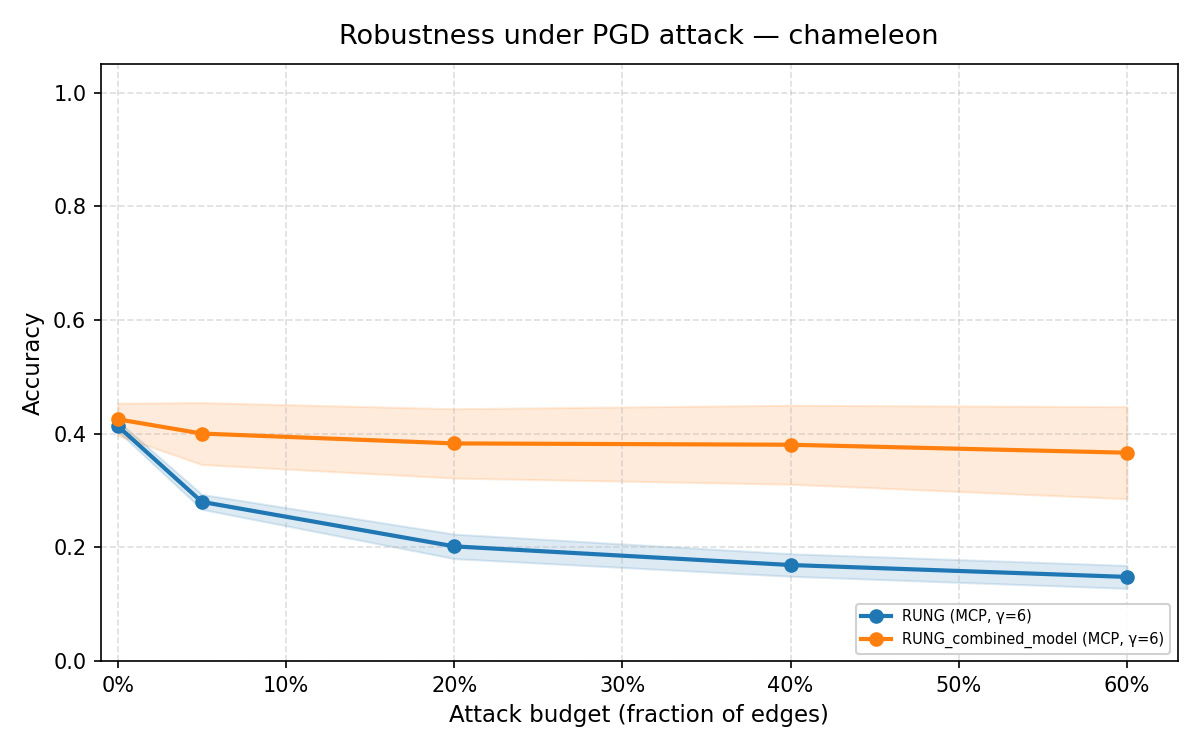
\includegraphics[width=\linewidth]{figures/Chameleon_RUNG_vs_RUNG_combined.jpg}
	\caption{Chameleon: RUNG vs Combined Model.}
	\Description{Comparison plot on Chameleon between baseline RUNG and combined method.}
	\label{fig:chameleon_combined}
\end{figure}

\begin{figure}[!htbp]
	\centering
	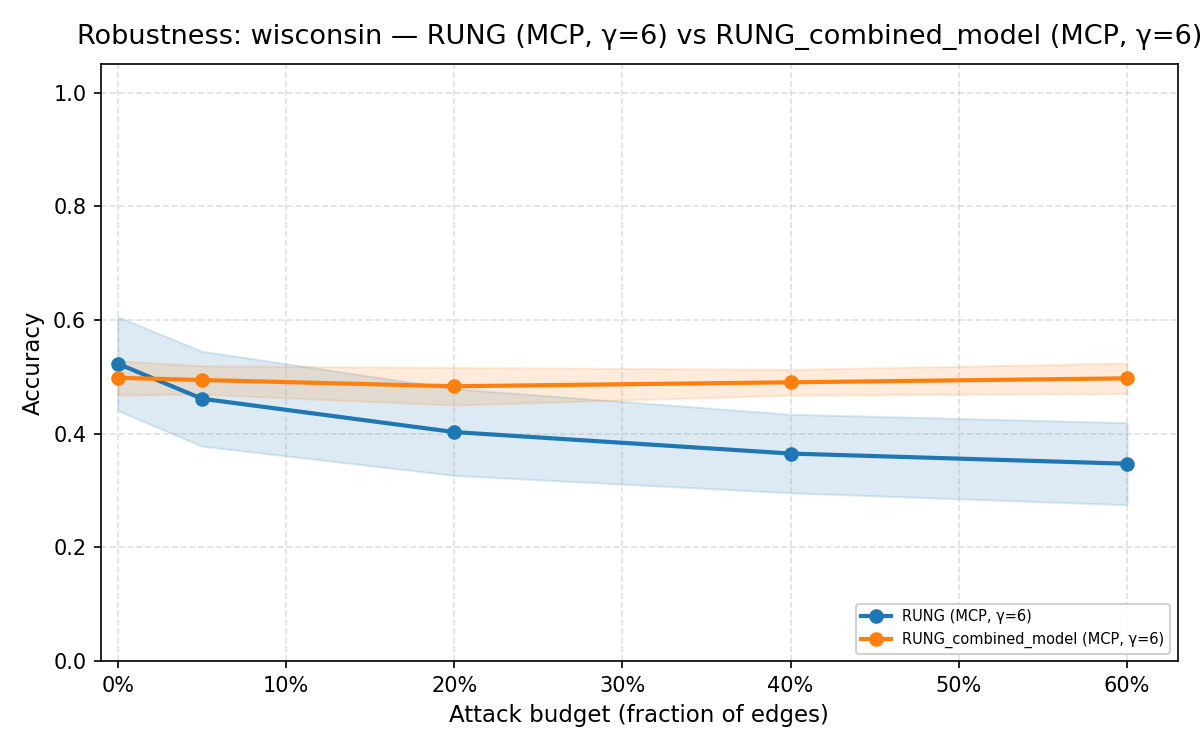
\includegraphics[width=\linewidth]{figures/Wisconsin_RUNG_vs_RUNG_combined.jpg}
	\caption{Wisconsin: RUNG vs Combined Model.}
	\Description{Comparison plot on Wisconsin between baseline RUNG and combined method.}
	\label{fig:wisconsin_combined}
\end{figure}

\begin{figure}[!htbp]
	\centering
	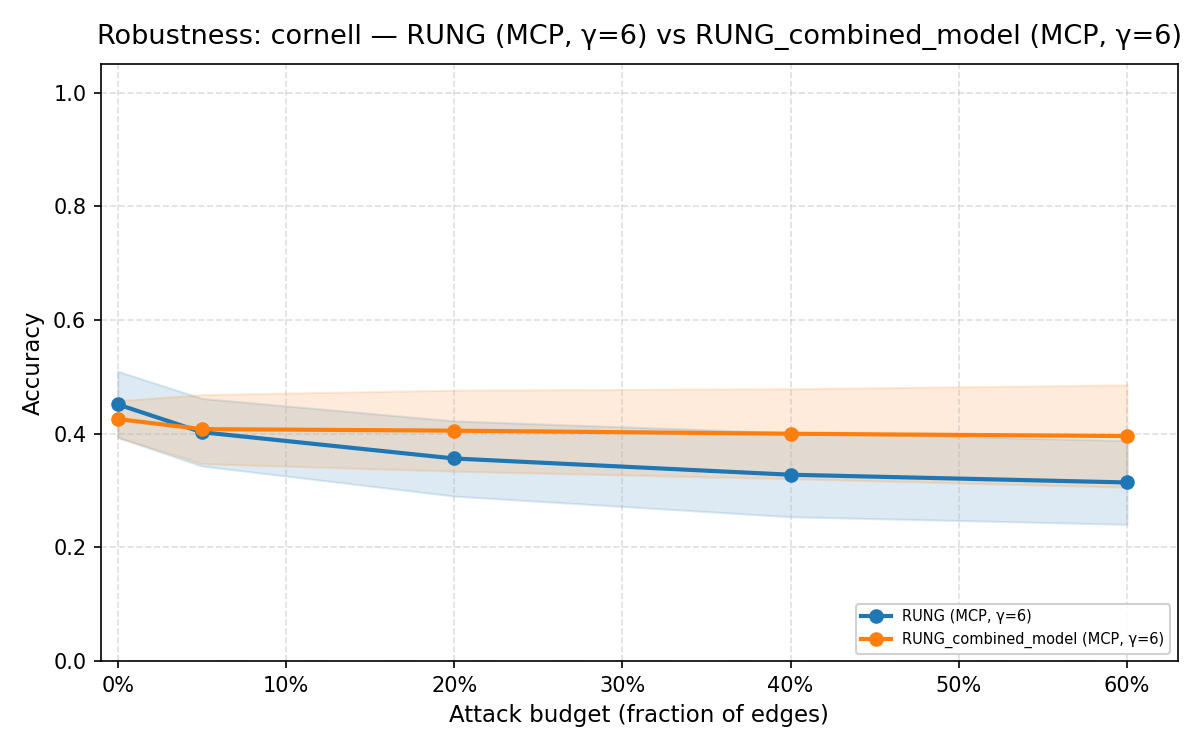
\includegraphics[width=\linewidth]{figures/Cornell_RUNG_vs_RUNG_combined.jpg}
	\caption{Cornell: RUNG vs Combined Model.}
	\Description{Comparison plot on Cornell between baseline RUNG and combined method.}
	\label{fig:cornell_combined}
\end{figure}

\subsection{Heterophilic Graph Analysis}
The paper itself already indicates that RUNG is mainly designed for homophilic graphs. That is why we included Chameleon, Wisconsin, and Cornell \cite{pei2020geomgcn}. In our tests, baseline RUNG performs weakly in these settings. Learnable Cosine Distance often performs better, likely because Euclidean distance fails when valid neighbors are far in magnitude but still structurally meaningful.

\begin{figure}[!htbp]
	\centering
	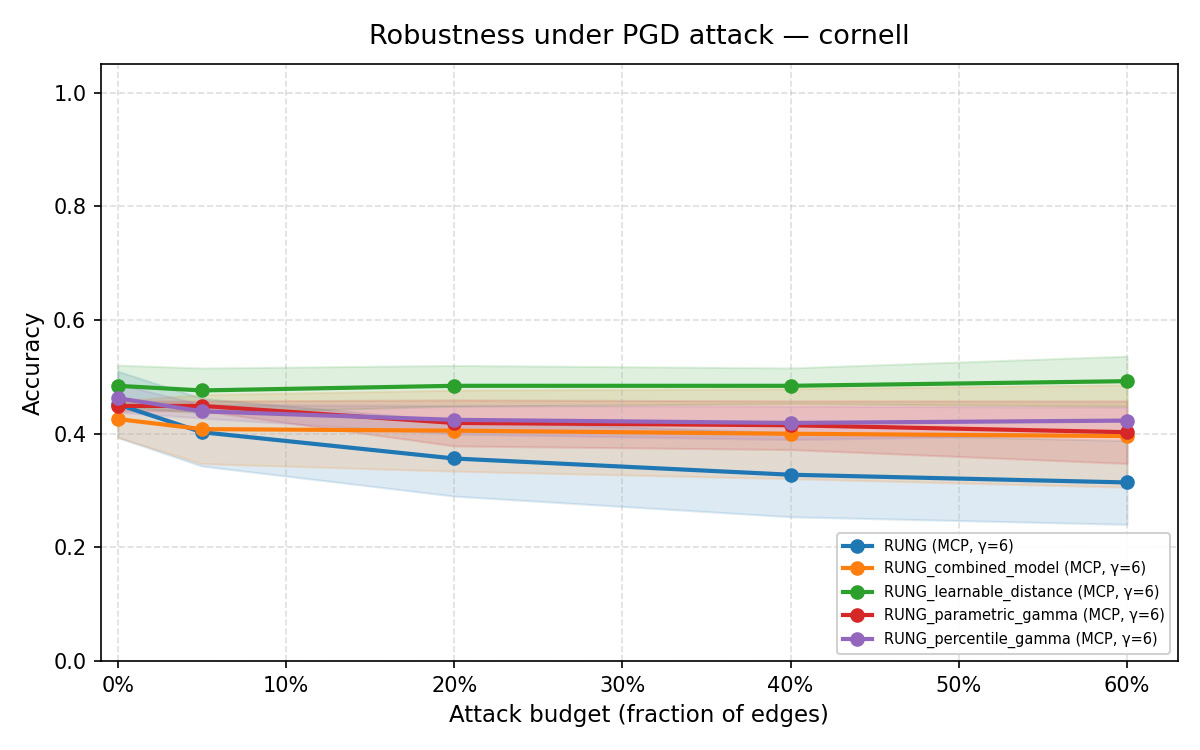
\includegraphics[width=\linewidth]{figures/Cornell_All.jpg}
	\caption{Cornell: All methods comparison.}
	\Description{Full comparison plot for Cornell including multiple methods in one figure.}
	\label{fig:cornell_all}
\end{figure}

\begin{figure}[!htbp]
	\centering
	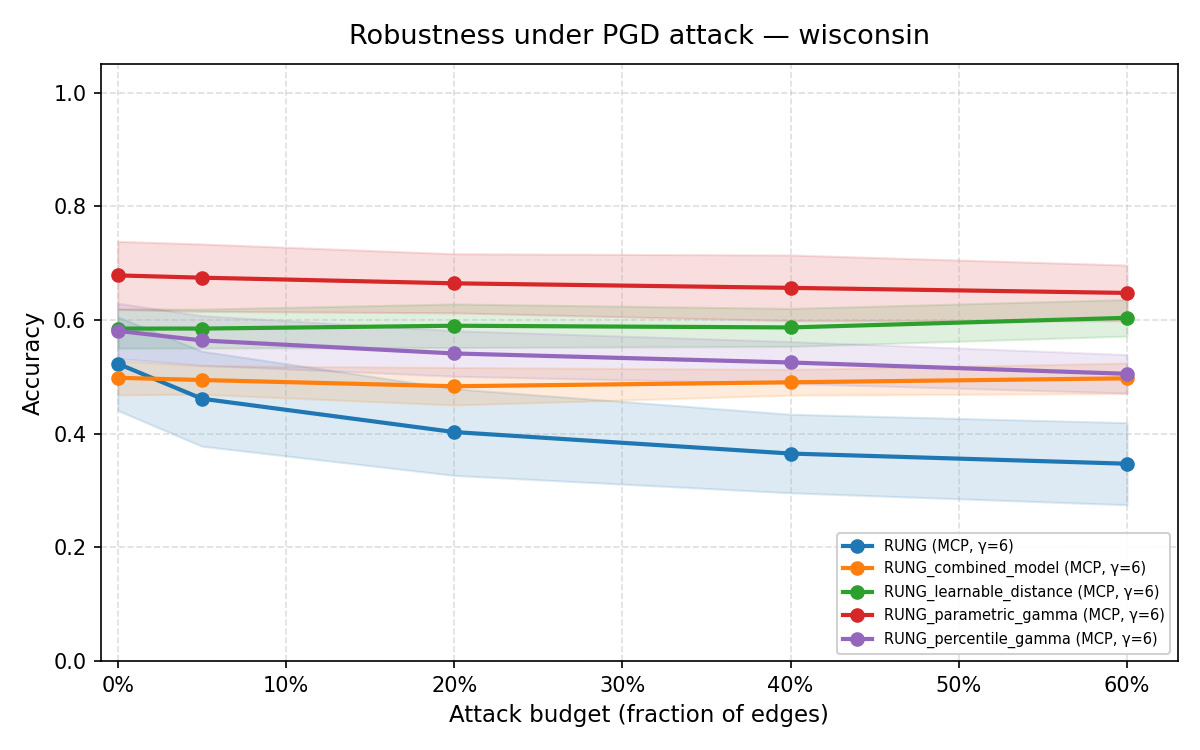
\includegraphics[width=\linewidth]{figures/WIsconsin_All.jpg}
	\caption{Wisconsin: All methods comparison.}
	\Description{Full comparison plot for Wisconsin including multiple methods in one figure.}
	\label{fig:wisconsin_all}
\end{figure}
\FloatBarrier

The core issue we observed is a double-correction effect in heterophilic graphs. Learnable Distance tries to balance directional structure, but depth-wise parametric strictness can increase pruning too quickly. This can choke message passing and remove valid heterophilic edges. This explains why independent methods can beat the combined model in heterophilic space.

From this progress stage, our scientific claim is the following:

\textit{Our experiments reveal that while a combined approach is highly effective for homophilic graphs, heterophilic graphs suffer from over-regularization when dynamic thresholding (Percentile/Parametric) is combined with dynamic metrics (Learnable Distance). For heterophilic environments, upgrading the distance metric to Cosine Learnable Distance independently yields the most optimal robustness, as it prevents the accidental over-pruning of valid heterophilic edges.}

\section{Conclusion}
This progress report shows that our three modifications improve robustness over base RUNG in many attack settings. Percentile Gamma and Parametric Gamma address depth-wise threshold mismatch caused by oversmoothing. Learnable Cosine Distance improves robustness by changing edge suspiciousness measurement from magnitude-driven Euclidean comparison to direction-aware similarity.

The combined model performs strongly on homophilic datasets, especially under high attack budget. For heterophilic datasets, we observed that independent Learnable Cosine Distance can outperform the combined setup because strict dynamic pruning can remove valid edges.

For future work toward the final project presentation, we plan to:
\begin{itemize}
\item complete broader training and testing for each method independently and in combination,
\item increase attack budget analysis beyond current levels up to 100\%,
\item build stronger variance analysis plots for all datasets,
\item and develop clearer theoretical guarantees for why each method behaves this way.
\end{itemize}

The theoretical part is still hard for us because the base paper is complex and these topics are new to us, but this is the key target before final presentation.

\bibliographystyle{ACM-Reference-Format}
\bibliography{references}

\end{document}
